% Master thesis - Mestrado em Informatica e Sistemas
% Luís Jordão
% Instituto Superior de Engenharia de Coimbra
% 2020/2021


% Packages

\documentclass[12pt,twoside]{report}
\usepackage[utf8]{inputenc}
\usepackage[a4paper,width=150mm,top=25mm,bottom=25mm,bindingoffset=6mm]{geometry}
%\usepackage[lmargin=25mm,rmargin=25mm,tmargin=27mm,bmargin=30mm]{geometry}
\usepackage[onehalfspacing]{setspace}
\usepackage[T1]{fontenc}
\usepackage[english]{babel}
\usepackage{emptypage}
\usepackage{graphicx,xcolor,comment,enumerate,multirow,multicol,indentfirst}
\usepackage{amsmath,amsthm,amsfonts,amssymb,dsfont,mathtools}
\usepackage{blindtext}
\usepackage{bibentry} 
\usepackage{longtable}
\usepackage{array}
\usepackage{url}
\usepackage{hyperref}
\usepackage[nottoc]{tocbibind}
\usepackage{hyphenat}
\usepackage{verbatim}
\usepackage{microtype}
\usepackage{kantlipsum}
\usepackage{subfigure}
\usepackage{float}
\usepackage{pdfpages}
\usepackage{xcolor}
\usepackage{fancyvrb}
\usepackage{multirow}

% ---- Blank page command ---- %
\usepackage{afterpage}
\newcommand\myemptypage{
    \null
    \thispagestyle{empty}
    \addtocounter{page}{-1}
    \newpage
}

% ---- Print XML code ---- %
\usepackage{listings}

\usepackage{color}
\definecolor{gray}{rgb}{0.4,0.4,0.4}
\definecolor{darkblue}{rgb}{0.0,0.0,0.6}
\definecolor{cyan}{rgb}{0.0,0.6,0.6}

\lstset{
  basicstyle=\ttfamily\small,
  columns=fullflexible,
  showstringspaces=false,
  commentstyle=\color{gray}\upshape,
  frame = single,
  numbersep=6pt,
  numbers=right
}

\lstdefinelanguage{XML}
{
  morestring=[b]",
  morestring=[s]{>}{<},
  morecomment=[s]{<?}{?>},
  stringstyle=\color{black},
  identifierstyle=\color{darkblue},
  keywordstyle=\color{cyan},
  morekeywords={xmlns,version,type}% list your attributes here
}

% Header and Footer
\usepackage{fancyhdr}
\pagestyle{fancy}

\fancyhead[LO,RE]{Chapter \thechapter}
\fancyhead{}
\fancyfoot{}
\fancyfoot[RO,LE]{\thepage}
\fancyfoot[LO]{Luís Miguel Coelho Jordão}
\fancyfoot[RE]{Mestrado em Engenharia Informática}
%\leftmark
%\rightmark 
\renewcommand{\headrulewidth}{0.8pt}
\renewcommand{\footrulewidth}{0.8pt}

% Document Begin
\begin{document}


% ---------- Document head starts ---------- %
% Include Chapters
\thispagestyle{empty}


\includegraphics[width=5cm]{images/logo-isec-transparente.png}

\begin{flushright}
{\Large{\textsl{Mestrado em Engenharia Informática}}}
\end{flushright}

%\hrulefill  %faz uma linha horizontal 

\rule[0.5ex]{35em}{0.5ex}
\vspace{2ex}

\begin{flushright}
{\LARGE{\textbf{\textsl{Automatic Test Definition for High-Integrity Systems}}}}\\
\vspace{4ex}
{\large{\textsl{Relatório de Projecto apresentado para a obtenção do grau de Mestre em Engenharia Informática}}}\\
\vspace{6ex}
{\normalsize{\textsl{\textbf{Autor}}}}\\
\vspace{1ex}
{\large{\textsl{\textbf{Luís Miguel Coelho Jordão}}}}\\
\vspace{6ex}
{\normalsize{\textsl{\textbf{Orientadores}}}}\\
\vspace{1ex}
{\large{\textsl{\textbf{Professor Doutor João Cunha}}}}\\
\vspace{1ex}
{\large{\textsl{Professor do Departamento de Engenharia Informática e Sistemas}}}\\
\vspace{1ex}
{\large{\textsl{Instituto Superior de Engenharia de Coimbra}}}\\
\vspace{6ex}
{\normalsize{\textsl{\textbf{Co-Orientador}}}}\\
\vspace{1ex}
{\large{\textsl{\textbf{Professor Doutor João Gabriel Silva}}}}\\
\vspace{1ex}
{\large{\textsl{Critical Software, SA}}}\\
\end{flushright}
\vspace{10ex}

\begin{center}
{\large{\textsl{\textbf{Coimbra, 2021}}}}\\
\end{center}

\clearpage


\newpage
\clearpage
\myemptypage

% Start Roman Numbering
\pagenumbering{roman}
% Needed to add Initial chapters to the table of contents
\addcontentsline{toc}{chapter}{Acknowledgments}
\chapter*{Acknowledgments}

Agradecimentos
\addcontentsline{toc}{chapter}{Resumo}
\chapter*{Resumo}

Resumo
\addcontentsline{toc}{chapter}{Abstract}
\chapter*{Abstract}
\label{ch:abstract}

Software and system testing is an intrinsic activity in software development. It is estimated that a great effort in the development of a system lies in the verification and validation of it. The scope of this report is the development of a tool capable of generating sets of test cases by interpreting software requirements written in a predefined format, thus allowing to greatly reduce the costs associated with the testing activities.\\
Sesnando is a tool developed at Critical Software, S.A. whose objective is to interpret and compile requirements written in a controlled natural language and from these, automatically generate a set of tests or test specification that allow verifying the realisation or implementation of this same requirement. During the interpretation phase of the given requirement, \textit{Sesnando} acts as a validator for writing the requirement and provides messages to the user about its construction. On a successful compilation, \textit{Sesnando} connects to a remote service to obtain additional information about the requirements. The test specification generated by \textit{Sesnando}, that contains the definition of the values of the signals to be assigned in the system as well as the expected results (observation of the behavior of the system), also in the form of signals (signal read) is composed of test steps. Each test step writes and reads a set of system signals. The set of these test steps is generated according to the test coverage criteria that must be applied, in this case the MCDC. The results obtained show that it is possible to reduce the effort in the system testing activity by up to 90\% per requirement.






% Table of contents
\tableofcontents
% List of Figures
\listoffigures
% List of tables
\listoftables

\addcontentsline{toc}{chapter}{Acronyms}
\chapter*{Acronyms}

%\begin{table}[h!] %\footnotesize
    \setlength{\LTleft}{0pt}
    \begin{longtable}{l l}
    \textbf{ANTLR}      &   ANother Tool for Language Recognition\\
    \textbf{API}        &   Application Programming Interface\\
    \textbf{ASDT}       &   Aerospace, Defense and Transportation\\
    \textbf{AST}        &   Abstract Syntax tree\\
    \textbf{CCTV}       &   Closed-Circuit Television\\
    \textbf{CNL}        &   Controlled natural language\\
    \textbf{CSW}        &   Critical Software\\
    \textbf{GUI}        &   Graphical User Interface\\
    \textbf{GWT}        &   Given-When-Then\\
    \textbf{ICD}        &   Interface Control Document\\
    \textbf{ISEC}       &   Instituto Superior de Engenharia de Coimbra\\
    \textbf{IV\&V}      &   Independent Verification and Validation\\
    \textbf{JRU}        &   Juridic Recording Unit\\
    \textbf{MCDC}       &   Modified Condition / Decision Coverage\\
    \textbf{MEI}        &   Mestrado em Engenharia Informática \\
    \textbf{NLP}        &   Natural Language Processing \\
    \textbf{PIBS}       &   Passenger Information and Beacon System \\
    \textbf{SIL}        &   Safety Integrity Level \\
    \textbf{SRS}        &   Software Requirements Specification \\
    \textbf{TCMS}       &   Train Control and Management System \\
    \textbf{VnV}        &   Verification and Validation \\
    \end{longtable}
    \label{tab:my_label}
%\end{table}

% ---------- Document head ends ---------- %

% To start arabic numerals
\pagenumbering{arabic}

% ---------- Document main sections ---------- %
%----------------------- Introduction ----------------------------
\chapter{Introduction}
\label{ch:1}


By mid-1968 the term Software Engineering was coined at NASA by Margaret Hamilton \cite{first_sw_engineer}. During that time more than 400 people were working on Apollo’s software, because software was how the US was going to win the race to the moon. As it turned out, of course, software was going to help the world do so much more \cite{mcmillan_her_nodate}. 

At that time, programming meant punching holes in stacks of punch cards, which would be processed overnight in batches on a giant computer that simulated the Apollo lander’s work. Everything needed to be tested precisely \cite{mcmillan_her_nodate}.

One day, Margaret’s daughter was playing with the command module simulator’s display-and-keyboard unit and as she toyed with the keyboard, an error message popped up. Lauren had crashed the simulator by somehow launching a pre-launch program called P01 while the simulator was in mid-flight. There was no reason an astronaut would ever do this, but nonetheless, Hamilton wanted to add code to prevent the crash.

NASA denied this idea by stating that the astronauts were trained to be perfect and they would not make any mistakes. So Hamilton added certain procedures to the documentation stating what astronauts should and should not do. However, they did mistakes. In the late 1968, an astronaut inadvertently selected a functionality that had wiped out all the navigation data and without that data, the Apollo computer would not be able to figure out how to get the astronauts home. Fortunately, Houston uploaded new navigational data and the Apollo astronauts came home \cite{first_sw_engineer} \cite{mcmillan_her_nodate}.\\

% ----- NASA ends ----- %
\\Testing activities are within the most important tasks of any business, from the world of software to the toothpaste we use, which should be meticulously tested to guarantee quality before being placed in the hands of the user. The objective of this phase is to guarantee quality standards to avoid failures in the product that might lead to catastrophic losses. \textcolor{red}{One of the reasons why this market keeps growing is due to the high costs involved in correcting these failures in advanced stages, however, detecting them in early stages is very profitable \cite{hernandez_history_2020}.
\\ //TODO: Refrasear este paragrafo. Dizer que existe mercado em torno de bugfixing e que detectar os problemas o mais cedo possivel após estes serem introduzidos é o ideal. e depois ver se há alguma coisa na frase que possa ser mantida e que faça sentido.}


% ----- testing ends ----- %

\textcolor{red}{Software requirements play an essential role when designing a system. Requirements are descriptions of how a software product should perform and therefore, should include not only user needs but also those arising from general organizational, government and industry standards \cite{aurum_engineering_2005}.}

The objective of this project is to create a compiler capable of understanding Functional Requirements and automatically generate their test cases. 

\textcolor{red}{
In order to use this application, such software requirements shall be written on a controlled natural language (CNL) that define the functionalities of a software system. This compiler aims to automatically generate high-level tests by parsing and interpreting requirement contents into a Parse tree. Unit tests are not in the scope of the current project. \\
//todo: Isto pode muito bem ser uma intro de uma próxima secção.
}

%----------------------- Problem and Motivation ----------------------------
\section{Problem and Motivation}
\label{sec:problem_and_motivation}

Common requirements engineering activities involve elicitation, interpretation and
structuring (analysis and documentation), negotiation, verification and validation,
change management and requirements tracing. There are several process models
available to describe the requirements engineering process. The process itself is
often depicted in different forms, including linear, incremental, non-linear and spiral models \cite{aurum_engineering_2005}.
Despite the effort to produce requirements, requirement testing can also be a costly and challenging activity. IV\&V teams are independent of the development organization on a technical, managerial, financial, and contractual basis, but have well-established, working relationships with the development organization \cite{noauthor_independent_2013}. Verification and Validation teams are required to gather solid knowledge about software systems and learning technical features and operational concepts on complex systems such as Trains, Satellites or in the area of Avionics can take several time to master. A misunderstood requirement or lack of technical domain can result in tests that fail or in countless hours of back-and-forth communication.
To address this problem, it was thought of a system to store common technical knowledge and capable of automatically generate test specifications given any software requirement as an input.


%----------------------- Objectives ----------------------------
\section{Objectives}
\label{sec:objectives}
It is known that good textual requirements are critical for the creation of successful systems, and heavy and vague natural language is highly discouraged \cite{incose}.
One of the roles of this software program is to guarantee that the requirements of the system under testing are following a predefined grammar [See Section 3] by checking their syntax and whether they are parseable, otherwise, a syntax-error message is generated. On a side note, having the written requirements following a stipulated grammar makes those requirements much easier to understand by the test engineers.
When the requirements are successfully parsed, the conditions and expected results are extracted from them. The required data, to support the test generation process is stored on a knowledge-base in a form of a software signal database.


%----------------------- Schedule ----------------------------
\section{Schedule}
\label{sec:schedule}
This project has been composed by five main activities. Those are illustrated on the following Figure \ref{fig:schedule}.

\begin{figure}[h]
    \centering
    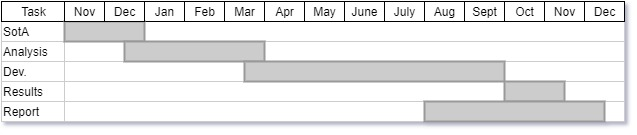
\includegraphics[width=\textwidth]{images/gantt.jpg}
    \caption{Scheduled Activities}
    \label{fig:schedule}
\end{figure}

\begin{itemize}
    \item SotA - State of the art - Study of the existing technologies and scientific advances and how they can contribute to this project.
    \item Analysis - Analysis and problem dismantling - This task consisted of the analysis of the available resources, results from state of the art and \textit{Datasets} e.g. sets of requirements.
    \item Dev. - Development of the solution - Development of the application, capable of understanding requirements, generating test cases, and test artifacts.
    \item Results - Results and further testing - Analysis of the produced results from the developed tool as well as possible adjustments.
    \item Report - Final project Report - Writing a final project report containing the results from all previous phases.
\end{itemize}

\newpage
%----------------------- Starting point ----------------------------
\section{Starting point}
\label{sec:starting_point}

\textit{Sesnando} has kicked-off at Critical Software (CSW) under the management of Dr. João Gabriel Silva. When the current thesis works have started to be carried out, a Railway project was being developed at CSW in increments and in a stable phase, given that it was already operating in passenger service. It has been decided to evaluate the capabilities of \textit{Sesnando} against such project.\\
A new grammar has been designed, specified, accepted and implemented to accomodate the requirements of the target Railway Project. Test Generator and Test Designer have been created under the scope of this thesis and the overall solution evolved to scalable architecture, so that, it can be easily adapted to future projects.
Signal Manager has been developed at CSW by a graduate engineer where several talks have been carried-out about its architecture and design in order to create a consensus with the test generation module.


%----------------------- Scope of this doc ----------------------------
\section{Scope of this document}
\label{sec:document_scope}

The first chapter (Ch. \ref{ch:1}) introduces the current project, its main motivations and objectives in general.\\
The second chapter (Ch. \ref{ch:2}) presents the limitation of this study and how it was conducted.\\
The third chapter (Ch. \ref{ch:3}) presents the state of the art, what are the current scientific advances in this subject, the available tools and technology.
The forth chapter (Ch. \ref{ch:4}) discusses the works done for this project, its requirements and architecture, and it's divided on two main sections, the application life-cycle and the method. The former (Sec. \ref{sec:application_lifecycle}) presents \textit{Sesnando} on a higher level and describes the main functionalities of the software and how to operate it. The latter (Sec. \ref{sec:method}) presents the project in a lower perspective, how its core functionalities have been implemented and the reasons behind it.
The fifth chapter (Ch. \ref{ch:5}) presents the conclusion and the final results from the analysis of this tool in-the-field.

\label{ch:2}
\chapter{Limitations of this study}

This software application will be firstly focused on a mature railway project where already advanced development has been made. Its requirements will be used as a mold for the creation of the predefined grammar of the acceptable requirements by the application under development (SESNANDO). It is intended to develop a core grammar that can interpret requirements from multiple railway projects. However, at the current state of the development made, using SESNANDO for a different project might require a slightly modified grammar to be created and installed. \\

By the time the developments of this software application started, there were already a significant number of requirements written on the company's client side involving natural language that were not precisely aligned with the internal defined guidelines. For the verification of this tool, such requirements needed to be re-written in a format that SESNANDO could interpret them.\\

It is intended (as discussed internally) that this software could be used on a railway project for Infraestruturas de Portugal. By the time of the writing of this report, this project is still in early development days, thus, for the validation of this tool, and as the scope of this thesis the former railway project will be used.\\

\chapter{State of the art}
\label{ch:sotart}

STATE OF THE ART\\
o que existe no mercado\\
porque é que não serve\\
o que se pretende optimizar\\
porque é que o sesnando vai ser melhor.


This section presents the study of the technology and the concepts contained within this project, as well as some of the already existing solutions. \textit{Sesnando} interprets software requirements written in a controlled natural language using computational linguistics and language recognition techniques. Tests for these requirements are then generated by applying software testing algorithms.

There are several techniques to derive test cases from functional
requirements. A similar approach has been researched by ... where









%----------------------- Software requirements ----------------------------
\section{Software Requirements}
\label{sec:software_requirements}

Software Requirements are a set of statements contained on a Software Requirements Specification (SRS) document that describe a system behaviour or functionality. Usually, software requirements are a low-level design of the business requirements. 

\textcolor{blue}{Software requirements play an essential role when designing a system. Requirements are descriptions of how a software product should perform and therefore, should include not only user needs but also those arising from general organizational, government and industry standards \cite{aurum_engineering_2005}.}

Extremely accurate requirements are hard to define, as such, some principles have been designed to ease this process, e.g. the \textit{INCOSE Guide for Writing Requirements} \cite{incose} or the \textit{S.M.A.R.T} criteria \cite{mannion_smart_2004} in order to improve how they are written, so they are strongly understandable by a human or a machine.\\
Requirements are written prior to the development phase and are usually written by the Developers and Requirement Managers. Errors introduced during the Requirements Engineering phase have exponential costs on later phases, therefore, the importance of writing precise requirements. \\
Error-free requirements are the foundations on which the code should be build and which the code should be tested. If the requirements are faulty, the code is likely to be faulty and tests of the code will be impossible, will fail, or give meaningless results. The effort to produce error-free requirements is considerable, but is nevertheless smaller that the effort to answer questions and to correct the requirements, the code and its tests because the original requirements were faulty.



\subsection{Requirement Specification Techniques}
\label{subsec:requirement_specification}

Behaviour Driven Development\\
Test-Driven Development (foco no facto do desenvolvimento ser orientado aos testes e não aos requisitos)\\
Describe the Gherkin language.\\
Sesnando uses the gherkin language structure.\\
The gherkin language defines the main requirement skeleton\\
Given são pre-condições, When representa uma mudança de estado ou trigger, Then representa como o sistema ou software se deve comportar\\


\section{Computational Linguistics and Language Recognition}
\label{sec:computational_linguistics}


Chomsky types\\
chomsky types 0 to type 3\\
LTR and LL(*)\\
bottom-up and top-down\\
lexers\\
parsers\\
Falar do ANTLR\\
Explicar o que é uma AST\\
Explicar o que é o antlr\\
porquê o antlr\\

%----------------------- Software testing ----------------------------
\section{Software testing}
\label{sec:software_testing}

The purpose of software testing activities is to verify that a system is operating according to predefined design and meets the customer needs.
Testing can occur on different levels 
\\
\textcolor{red}{
Notes:\\
what is the purpose of testing activities\\
who should be testing\\
who writes tests\\
why are tests so important ... (without tests the software would be prone to errors)\\
FALAR DO V-MODEL\\
introduzir paths and branchs
}


\subsection{Black-box testing}
\label{subsec:black-box testing}

Cause-Effect graph 


\section{Requirement Testing Tools}
\label{subsec:requirement_testing}

Cucumber\\
Cucumber is a tool that supports behaviour-driven development. It reads Test definitions and test steps written using the Gherkin language \cite{cucumber}.\\

Jest\\
Cypress\\

%----------------------- Software testing ----------------------------
\section{Related Works}
\label{sec:related_works}

Artigos\\

%----------------------- Current procedures ----------------------------
\section{Overview of the current industry procedures}
\label{sec:current_procedures}

This section presents the system testing activities in which critical software is involved.
The process begins when the rolling stock manufacturer receives a set of customer requirements commonly known as \textit{Business requirements}. Aside from these requirements, there are the Rule book requirements which are documents that contain direct instructions to Railway staff, as well as the requirements from the \textit{standards} catalogues related to a Safety Integrity Level (SIL). SIL levels go from level 0 to level 4 according to the critically of a system being SIL4 systems less prone to fail. There are several \textit{standards} catalogues applicable to the railway industry, the norms applicable to software design on vehicle systems is EN 50126 \cite{en50126} and EN 50126 \cite{en50128}. From these requirements, new architectural, performance, functional and sub-system requirements are created.\\

\textcolor{red}{o que é que o 126 define e o que o 128 define... falar de RAMS?}

The functional team, responsible of Functional requirements, needs to assure that these derived requirements satisfy the original customer requirements, are testable, coherent and non-contradictory. The development team writes software requirements derived from functional level and implements the software following the norm EN 61131 \cite{en61131}. To facilitate code safety, Ada language and Misra-C are also used at critical software in the area of Aerospace, Defense and Transportation (ADST).\\

The software is only uploaded to vehicle level once all tests under the system level are verified under a simulated environment in the form of a \textit{Test Rack} for SIL requirements, containing all safety devices like the Central Control Unit of the train or in a form of a virtual environment installed on the testers' computer for non-SIL requirements (SIL-0). \\

The activity of testing relies on the interpretation of the software requirements stored on a IBM DOORS database by the manufacturer, and by verify if the system is behaving accordingly. To support the testing activities at system testing level, an Interface Control Document (ICD) is required. The purpose of the ICD is to support the information present on a requirement by mapping its conditions to one or more software signals, which are the internal logic of the Train Control and Management System (TCMS) and might act from a simple button press to the representation of the status of a train door.\\

The realisation of testing a requirement relies on the identification of software signals that represent the logic present on a requirement e.g. the command to open a train door, passenger emergency button, etc. and on the definition of the combination between the inputs and expected results in order to meet the requirement coverage criteria. This combination of test steps results in a test specification that can be converted into a test script using a test tool provided by the manufacturer. The test script is then loaded on the test tool which will then produce a test report file. Tests might by automatic or semi-automatic depending on the nature of the system. 


\section{Conclusions on state of the art}
\label{sec:sota_conclusions}

Alguns artigos lidos tentam chegar à interpretação de linguagem natural, que pode induzir em erro, ou definem uma linguagem natural controlada mas dependem de muitos inputs do utilizador, outros artigos pedem ao utilizador para atribuir significado às palavras na altura do processamento do requisito.


\chapter{Sesnando}
\label{ch:4}

This section introduces the SESNANDO project by describing the software operability and its core functionalities.

\section{Requirement analysis}
\label{sec:requirement_analysis}

The activity of identifying software functionalities and behavior is described as \textit{Requirements Engineering}. Before proceeding to the presentation of the SESNANDO architecture those will be identified in a simple manner.

\begin{itemize}
\item The application must be able to recognize a requirement identified by its keyword REQUIREMENT.
\item The application must be able to identify \textit{Given}, \textit{When} and \textit{Then} predicates.
\item The application must extract Logical Expressions between \textit{AND} and \textit{OR} boolean operators.
\item The application must identify Logical Expressions using the operators: \textit{Equal than}, \textit{Lower Than}, \textit{Lower Than or Equal}, \textit{Greater Than} and \textit{Greater Than or Equal}.
\item The application must be able to identify Requirement Signals (Logical Signals) within a Logical Expression.
\item The application must be able to identify an Operand within a Logical Expression.
\item The application must be able to identify a Logical Expression Quantifier, i.e., the system components to which the expression shall be evaluated, e.g., a train axle.
\item The application must be able to compile the requirement into a Parse tree.
\item The application must be able to access the Parse Tree and generate a set of test cases from the interpreted requirements.
\item The application must be able to generate a standard output file (CSV) containing a set of test cases.
\item The application must be able to generate a test script to be used on the testing environment.
\end{itemize}



\section{Software Architecture}
\label{sec:software_architecture}

Sesnando is divided into multiple modules that communicate with each other. Next those modules will be presented as well as their main roles within sesnando. \\

\begin{figure}[h]
    \centering
    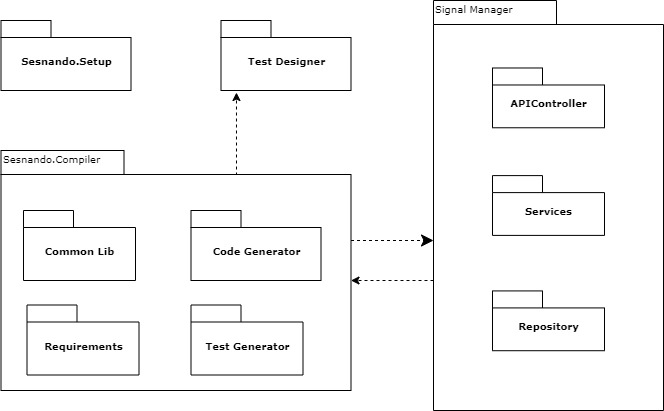
\includegraphics[scale=0.625]{images/sesnando_modules.jpg}
    \caption{Main application modules}
\end{figure}
\label{fig:sesnando_modules}

\begin{itemize}

\item Sesnando.Setup - Is responsible to verify and install all the Application dependencies on the operating system.

\item Sesnando.Compiler - Is the entry point of this Application and will call all the relevant modules as needed.

\item Requirement Module - This module will be called in the beginning of the program execution. It will read the input requirements and will then parse its contents using an Abstract Syntax Tree, i.e. it contains a predefined grammar that will be used to compile the requirement into a set of Objects. Those will be detailed further within this document.

\item Test Generator - Once the object tree is successfully constructed, this module will be notified to extract the required data from it in order to start to define the first tests, the Object tree will be then mutated to generate new test cases.

\item Common Lib - Where the actual Abstract Syntax Tree objects will be stored, accessible to the whole application suite.

\item Signal Manager - The conversion of the Input requirements into Object trees is not direct and trivial. Signal Manager is a detachable service that contains a database with the purpose to provide low-level technical context to the requirements, i.e., the requirement describe the functionalities on a high-level of abstraction which will be then mapped to a set of software signals ready to be used on the test environment. This is how the application can generate accurately software tests.

\item Code Generator - This module receives the standard output from the test generator and will then generate proper test artifacts compatible with the end test environment, e.g. test scripts.

\item Test Designer - Test designer is a detachable Graphical User Interface (GUI) module with the main purpose of displaying the generated test cases to the User. From this tool, the user is able to review, edit and export these test cases into a permanent file.
\end{itemize}

%----------------------- Software Architecture ----------------------------
\section{Software Architecture}
\label{sec:software_architecture}

Sesnando is divided into multiple modules that communicate with each other. Next those modules will be presented as well as their main roles within sesnando. \\

\begin{figure}[h]
    \centering
    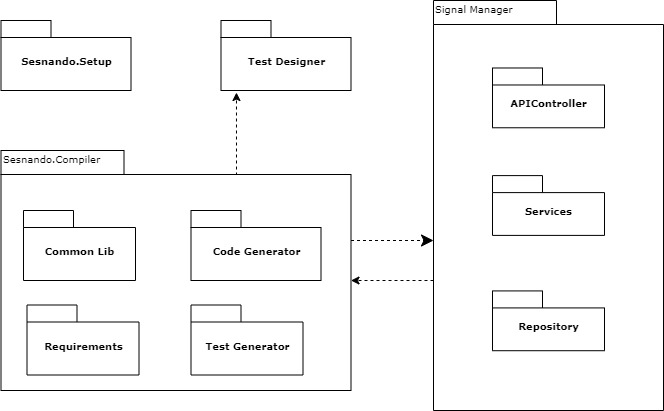
\includegraphics[scale=0.625]{images/sesnando_modules.jpg}
    \caption{Main application modules}
\end{figure}
\label{fig:sesnando_modules}

\begin{itemize}

\item Sesnando.Setup - Is responsible to verify and install all the Application dependencies on the operating system.

\item Sesnando.Compiler - Is the entry point of this Application and will call all the relevant modules as needed.

\item Requirements - This module will be called in the beginning of the program execution. It will read the input requirements and will then parse its contents using an Abstract Syntax Tree, i.e. it contains a predefined grammar that will be used to compile the requirement into a set of Objects. Those will be detailed further within this document.

\item Test Generator - Once the object tree is successfully constructed, this module will be notified to extract the required data from it in order to start to define the first tests, the Object tree will be then mutated to generate new test cases.

\item Common Lib - Where the actual Abstract Syntax Tree objects will be stored, accessible to the whole application suite.

\item Signal Manager - The conversion of the Input requirements into Object trees is not direct and trivial. Signal Manager is a detachable service that contains a database with the purpose to provide low-level technical context to the requirements, i.e., the requirement describe the functionalities on a high-level of abstraction which will be then mapped to a set of software signals ready to be used on the test environment. This is how the application can generate accurately software tests.

\item Code Generator - This module receives the standard output from the test generator and will then generate proper test artifacts compatible with the end test environment, e.g. test scripts.

\item Test Designer - Test designer is a detachable Graphical User Interface (GUI) module with the main purpose of displaying the generated test cases to the User. From this tool, the user is able to review, edit and export these test cases into a permanent file.
\end{itemize}

    %----------------------- Requirement analysis ----------------------------
\section{Requirement analysis}
\label{sec:requirement_analysis}

The activity of identifying software functionalities and behavior is described as \textit{Requirements Engineering}. Before proceeding to the presentation of the \textit{Sesnando} architecture, the requirements of the \textit{Sesnando} tool (denominated as 'The application') will be identified in a simple manner.

\begin{itemize}
\item The application must be able to recognize a requirement identified by its keyword REQUIREMENT.
\item The application must be able to identify \textit{Given}, \textit{When} and \textit{Then} predicates.
\item The application must extract Logical Expressions between \textit{AND} and \textit{OR} boolean operators.
\item The application must identify Logical Expressions using the operators: \textit{Equal than}, \textit{Lower Than}, \textit{Lower Than or Equal}, \textit{Greater Than} and \textit{Greater Than or Equal}.
\item The application must be able to identify Requirement Signals (Logical Signals) within a Logical Expression.
\item The application must be able to identify an Operand within a Logical Expression.
\item The application must be able to identify a Logical Expression Quantifier, i.e., the system components to which the expression shall be evaluated, e.g., a train axle.
\item The application must be able to compile the requirement into a Parse tree.
\item The application must be able to access the Parse Tree and generate a set of test cases from the interpreted requirements.
\item The application must be able to generate a standard output file (CSV) containing a set of test cases.
\item The application must be able to generate a test script to be used on the testing environment.
\end{itemize}
    \section{Functional Description}
%----------------------- Functional description ----------------------------
\label{sec:functional_description}

This section provides a detailed description of the internal building blocks of Sesnando.

\begin{itemize}
\item Command Line Arguments (Section \ref{subsec:command_line_arguments}) - presents the arguments that \textit{Sesnando} supports from the command line.
\item Input requirements (Section \ref{subsec:sesnando_input}) - Presents examples of the requirement structure that \textit{Sesnando} supports.
\item Requirement processing (Section \ref{subsec:requirement_processing}) - Presents the compilation of the requirement into a Parse tree and how a XML sample can be obtained by using Debug mode.
\item Grammar Elements (Section \ref{subsec:grammar_elements}) - Presents the installed grammar on \textit{Sesnando} and how requirements should be defined.
\item Signal Mapping (Section \ref{subsec:signal_mapping}) - Presents how Requirement signals are translated into Software signals.
\item Test Generation (Section \ref{subsec:test_generation}) - Presents how \textit{Sesnando} compiles input requirements and how tests are generated on a design level.
\item Signal Manager (Section \ref{subsec:signal_manager}) - Presents the main role of Signal manager on test generation and overview of its user interface.
\item Test Designer (Section \ref{subsec:test_designer}) - Presents the test designer user interface, and how test specifications are visualised with the aid of this module.
\end{itemize}


\subsection{Command Line Arguments}
%----------------------- Command Line Arguments ----------------------------
\label{subsec:command_line_arguments}

At the moment, Sesnando operates as a command line application. The command line arguments can be passed at the application launch, but a configuration file can be set, so that the user can define a set of default parameters avoiding the need to pass the arguments at all times. Default values from the configuration file will be used when omitting these parameters from the command line. The available command line arguments are defined on Table \ref{tab:CLI}.

As \textit{Sesnando} can be executed following a set of parameters from the command line or from a \textit{JSON} configuration, a detailed description of these commands are as follows.

\begin{itemize}
    \item signal\_manager - The address of the remote Signal Manager server, containing the data required to successfully generate test cases. Default port 5001.
    \item input - The location of the input file containing the requirements to be parsed by \textit{Sesnando}.
    \item output\_folder - The default location for the artifacts generated by \textit{Sesnando} (Can be overriden using "Save as..." from the test designer).
    \item test\_designer - The location of the Test Designer GUI module (usually on the same folder as the compiler binaries).
    \item debug - Debug mode mode allows a verbose execution of \textit{Sesnando}.
    
\end{itemize}

\begin{table}[H]
\caption{Sesnando Config parameters}
    \footnotesize
    \centering
    
    \begin{tabular}{c c c}
        \hline
        % --- ROW 1 --- %
        \textbf{\textit{Command}} & 
        \textbf{\textit{Default Value}} & 
        \textbf{\textit{Description}}\\ \hline  \\
        
        % --- ROW 2 --- %
        \begin{tabular}[c]{@{}c@{}} \textbf{\textit{-sm }} \textbf{\textit{--signal\_manager}}\end{tabular} & 
        127.0.0.1 & 
        Signal Manager IP Addr.\\
        \hline \\
        % --- ROW 3 --- %
        \begin{tabular}[c]{@{}c@{}} \textbf{\textit{-i }} \textbf{\textit{--input}}\end{tabular} & 
        ./input\_files/requirements.txt &
        Input Requirements location \\
        \hline \\
        % --- ROW 4 --- %
        \begin{tabular}[c]{@{}c@{}} \textbf{\textit{-o }} \textbf{\textit{--output\_folder}}\end{tabular} & 
        ./output\_files/ &
        Output Folder \\
        \hline \\
        % --- ROW 5 --- %
        \begin{tabular}[c]{@{}c@{}} \textbf{\textit{-td }} \textbf{\textit{--test\_designer}}\end{tabular} & 
        ./SESNANDO.TestDesigner.exe &
        Test Designer Location \\
        \hline \\
        % --- ROW 6 --- %
        \begin{tabular}[c]{@{}c@{}} \textbf{\textit{-d }} \textbf{\textit{--debug}}\end{tabular} & 
        N/A &
        Debug mode \\
        \hline \\
        
    \end{tabular}
    \label{tab:CLI}
\end{table}


\subsection{Input Requirements}
%----------------------- Input and Resources ----------------------------
\label{subsec:sesnando_input}

At this stage of the development, Sesnando takes a set of input requirements written in a text file (.txt) and parses them from there. These requirements must be compliant with a predefined grammar. The grammar specification is presented on Section \ref{subsec:grammar_elements}. The grammar guidelines \cite{sesnando-req-guidelines} has been documented by the author of the current thesis and was then reviewed and approved by the requirement managers at CSW. REQ442-1 is a simple example of a requirement structure that can be parsed by Sesnando.\\


\begin{Verbatim}[xleftmargin=12mm, numbers=left]
REQUIREMENT(REQ442-1, function, tcmsdevice) 
{
	GIVEN <RequirementSignal1> is equal to true
	    and <RequirementSignal2> is equal to true;
	WHEN;
	THEN <RequirementSignalX> is set to true;
}
\end{Verbatim}


\textit{GIVEN} and \textit{WHEN} predicates combined, dictate the outcome of the requirement. A concrete example of the above requirement is presented on REQ442-2.\\


\begin{Verbatim}[xleftmargin=12mm, numbers=left]
REQUIREMENT(REQ442-2, function, tcmsdevice) 
{
	GIVEN <Status Door Closing> is equal to true
	    and <Status of Obstacle Detection> is equal to true;
	WHEN;
	THEN <Door Obstacle Alarm and CCTV> is set to true;
}
\end{Verbatim}

As stated on the above requirement, when the GIVEN predicate evaluates to true, i.e, a Door is closing and an obstacle has been detected, the Train Control and Management System shall set a CCTV signal to true, so the incident can be visualised by the train driver.


\subsection{Requirement processing}
%----------------------- Requirement processing ----------------------------
\label{subsec:requirement_processing}

From the requirement examples at Section \ref{subsec:sesnando_input}, Sesnando uses a lexer and a parser (ANTLR Library \ref{sec:computational_linguistics}) to translate it into a Parse tree. A parse tree is a concrete representation of the input and contains all its information. Figure \ref{fig:req_parse_tree} is a representation of the Parsed requirement.
In order to use this application, such software requirements shall be written on a controlled natural language (CNL) that define the functionalities of a software system. This compiler aims to automatically generate high-level tests by parsing and interpreting requirement contents in this so called Parse tree.

\begin{figure}[H]
    \centering
    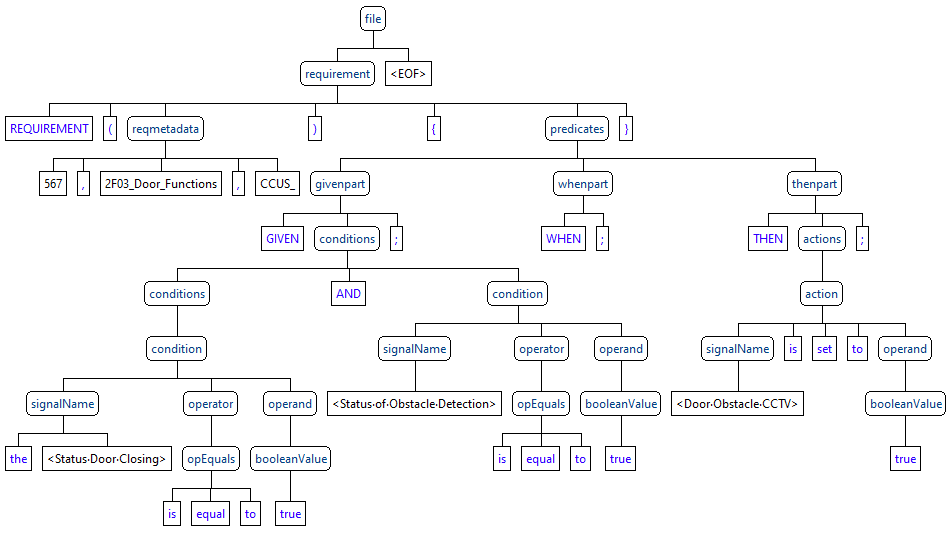
\includegraphics[scale=0.625]{images/parse_tree_req_example.PNG}
    \caption{Parse tree from the previous requirement example}
    \label{fig:req_parse_tree}
\end{figure}


Before executing \textit{Sesnando}, Debug mode can be enabled by setting the debug flag trough the command line. This will lower the Log level and \textit{Sesnando} will turn into a verbose execution by displaying the intermediate steps to the user. Due to this, \textit{Sesnando} provides a representation of the Parse tree in a form a XML structure: \\

\lstset{language=XML}
\begin{lstlisting}
<?xml version="1.0" encoding="utf-8"?>
<AST>
  <RequirementSet>
    <Requirement>
      <Id>123456</Id>
      <TestCaseId>R151_2F03_DoorStat_TC_001</TestCaseId>
      <Namespace>MWT_</Namespace>
      <GivenConditions p4:type="ComparisonExpression">
        <ExpressionType>EXP_COMPARISON</ExpressionType>
        <ExpressionOperator>
          <ExpressionType>EXP_COMP_OPERATOR</ExpressionType>
          <OperatorType>OP_EQ</OperatorType>
        </ExpressionOperator>
        <LogicalSignal>
          <ExpressionType>EXP_SIGNAL</ExpressionType>
          <SignalName>CTC_OPDoorsFromMIO</SignalName>
          <SignalFormat>SIGNAL_ALIAS</SignalFormat>
        </LogicalSignal>
        <SignalValue>
          <ExpressionType>EXP_SIGNAL_VALUE</ExpressionType>
          <Type>SV_BOOL</Type>
          <Value>TRUE</Value>
        </SignalValue>
      </GivenConditions>
      <WhenConditions p4:type="EmptyLogicalExpression">
        <ExpressionType>EXP_EMPTY</ExpressionType>
      </WhenConditions>
      <ThenActions p4:type="ActionExpression">
        <ExpressionType>EXP_ACTION</ExpressionType>
        <LogicalSignal>
          <ExpressionType>EXP_SIGNAL</ExpressionType>
          <SignalName>CTC_STrcnSafeFromMIO</SignalName>
          <SignalFormat>SIGNAL_ALIAS</SignalFormat>
        </LogicalSignal>
        <SignalValue>
          <ExpressionType>EXP_SIGNAL_VALUE</ExpressionType>
          <Type>SV_BOOL</Type>
          <Value>TRUE</Value>
        </SignalValue>
        <Actor />
      </ThenActions>
    </Requirement>
  </RequirementSet>
</AST>
\end{lstlisting}
\label{code:xml_output}

The above XML tree has been automatically generated by extending the Object class in C\# and defining a new \textit{ToXMLString()} method which then uses the native XML Serializer.\\
The corresponding Object Tree will be stored on the the SESNANDO.Compiler.Common module, making it available to the remaining modules via a controller class.


\subsection{Grammar Elements}
%----------------------- Grammar Elements ----------------------------
\label{subsec:grammar_elements}


One of the core values of \textit{Sesnando} is the ability to validate the writing of requirements given the installed grammar. This tool is able to display detailed error messages when it fails to interpret a given requirement as well as error messages when certain keywords or expressions are inadvisable. \\

Besides, the installed grammar tends to approach a level of natural language given that there is a tendency on these markets to describe high-level requirements using natural language as they are more readable by the stakeholders.

A requirement predicate is defined as a full set of clauses by each GIVEN or WHEN requirement elements, meaning each requirement contains two predicates, as those define the outcome of the requirement i.e. whether the THEN actions are applied or not. A requirement clause is a logical condition contained on each requirement predicate and are separated by boolean operators e.g. \textit{AND}s.
The most simple predicate (GIVEN or WHEN) clause contains two operands and an operator. The first operand is described as requirement signal and the second the signal value, which might be a boolean or an integer value. The most common operators are defined using natural language and are presented on Table \ref{tab:natural_operators}

\begin{table}[H]
\caption{Requirement grammar - common operators}
    \footnotesize
    \centering
    
    \begin{tabular}{c c}
        \hline
        % --- ROW Header --- %
        \textbf{\textit{Grammar Operator}} & 
        \textbf{\textit{Logical Operator}}
        \\ \hline  \\
        % --- ROW 1 --- %
        \begin{tabular}[c]{@{}c@{}} \textbf{\textit{ is equal to }} \end{tabular} & 
        = \\
        \hline \\
        % --- ROW 2 --- %
        \begin{tabular}[c]{@{}c@{}} \textbf{\textit{ is greater than }} \end{tabular} & 
        > \\
        \hline \\
        % --- ROW 3 --- %
        \begin{tabular}[c]{@{}c@{}} \textbf{\textit{ is greater than or equal to }} \end{tabular} & 
        <=\\
        \hline \\
        % --- ROW 4 --- %
        \begin{tabular}[c]{@{}c@{}} \textbf{\textit{ is lower than }} \end{tabular} & 
        <\\
        \hline \\
        % --- ROW 4 --- %
        \begin{tabular}[c]{@{}c@{}} \textbf{\textit{ is lower than or equal to }} \end{tabular} & 
        <=\\
        \hline \\
    \end{tabular}
    \label{tab:natural_operators}
\end{table}

As per Table \ref{tab:natural_operators}, an example of a clause containing a natural operator, could be defined as: \textit{GIVEN <Traction Safe Status> \textbf{is equal to} true in at least one DTCar in the train}.\\
This expression would check whether the requirement signal \textit{Traction Safe Status} evaluates to true on a given car of the train. A train usually contains 5 coupled cars.

\subsubsection{Quantifiers}
%----------------------- quantifiers ----------------------------
\label{subsubsec:quantifiers}

Each requirement predicate condition can be enhanced with a quantifier. A quantifier is useful when a requirement signal represents more than one element on the train of the same type, e.g. a train door, a train axle, brake mechanisms, etc. A quantifier defines how many or which elements of the same type need to fulfil a condition in order for the full clause (i.e., the base condition plus the quantifier) to evaluate to true.
Thus, a requirement signal can map to one or more technical signals. This will be presented on next Section \ref{subsec:signal_mapping}.\\

The following verbatim describes one of the system requirements. Right after, the actual requirement will be presented using the GWT blueprint.\\

\begin{Verbatim}[xleftmargin=12mm,numbers=left]
Given that a dragging brake is detected for at least one brake 
in the Train Unit, Dragging Brake Detected shall be set on the
Juridical Recording Unit.
\end{Verbatim}


\begin{Verbatim}[xleftmargin=12mm, numbers=left]
REQUIREMENT(REQ444-1, 2F02_Traction_Braking, CCUS)
{
	GIVEN <Dragging Brake Detected> is equal to true 
	    for at least one brake in the Unit;
	WHEN;
	// Juridical Recording Unit
	THEN <JRU Dragging Brake Detected> is set to true;
}
\end{Verbatim}

The above requirement written in the GWT blueprint defines that at least only one dragging brake is necessary for this event to be registered on the JRU. Line 6 of the second verbatim represents a comment that might be presented on the requirement to clarify any definition. This is supported by the installed grammar and will be ignored during the compilation of the requirement.\\

The complete list of the supported quantifiers is presented on the following bullet point list.

The following quantifier list is supported.
\begin{itemize}
    \item \textbf{FOR ONE} - Predicate clause evaluates to true if one and only one attribute/component within the quantifier evaluates to true, e.g. one of the two driver cabinets of the train.
        \begin{itemize}
            \item Example: <Status Train cab> is active \textbf{for one} cab of the train;\\
        \end{itemize}
    \item \textbf{FOR AT LEAST} - Predicate clause evaluates to true if at least one attribute/component within the quantifier evaluates to true, e.g. a door in a set of train doors.
        \begin{itemize}
            \item Example: <Status door> is open \textbf{for at least} one door of the train;\\
        \end{itemize}
    \item \textbf{FOR ALL} - Predicate clause evaluates to true if all attributes/components within
    the quantifier evaluates to true, e.g. all the emergency brakes need to be applied in order for the clause to evaluate to true.
        \begin{itemize}
            \item Example: <Status Emergency brake> is applied \textbf{for all} emergency brakes of the train;\\
        \end{itemize}
    \item \textbf{FOR THE SAME} <attribute/component> as in <Requirement Signal in FOR ONE quantifier>" - This quantifier must be used in conjunction with "for one" quantifier in the same requirement when both signals share the same attributes, i.e., the requirement signal within the clause containing the "for one" quantifier and the requirement signal within the "for the same..." quantifier. Predicate clause evaluates to true if the same attribute as in the "for one" clause contains the same attribute value. The following example describes a use case of this quantifier.
        \begin{itemize}
            \item Example: GIVEN <Train speed> is equal to 0 and <Door Locking> is equal to false;\\
                           WHEN <Driver Desk Door Open> is equal to true \textbf{for one} \textit{side} of the train;\\
                           THEN the <TCMS command door open> is set to true \textbf{for the same} \textit{side} as in <Driver Desk Door Open>; train;\\
        \end{itemize}
\end{itemize}

A requirement predicate supports multiple clauses and each clause supports only one quantifier. Each different quantifier is parsed into a different class object. Figure \ref{fig:quantifier_parse_tree} presents the following requirement containing a quantifier parsed into a Parse tree.


\begin{Verbatim}[numbers=left]
REQUIREMENT(REQ444-2, 2F03_Door_Functions, CCUS) 
{
	GIVEN <Status of Obstacle Detection> is equal to
	    true for at least one door of the train;
	WHEN;
	THEN <Door Obstacle alarm and CCTV> is set to true;
}
\end{Verbatim}
\label{req:door_obstacle_pt}

\begin{figure}[H]
    \centering
    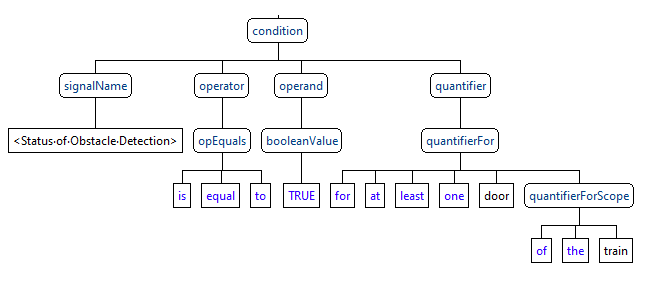
\includegraphics[scale=0.85]{images/quantifier_parse_tree.PNG}
    \caption{Requirement Quantifier Parse tree}
    \label{fig:quantifier_parse_tree}
\end{figure}


On Figure \ref{fig:quantifier_parse_tree}, for the quantifier node, "for at least one" defines the type of the quantifier. \textit{Door} is the component/attribute of the signal and the train is the scope of the signal (i.e., local car, unit, or the whole train), meaning that each Door needs to be checked whether the present conditions  evaluates to true for at least one door of the train (i.e., an obstacle has been detected during door close sequence).


\subsection{Signal Mapping}
%----------------------- Signal Translation ----------------------------
\label{subsec:signal_mapping}

The activity of automatic signal translation is integrated on Test Generator module as presented on Figure \ref{fig:data_flow} of Section \ref{sec:functional_overview}.\\
A requirement signal (Logical Signal) might map to one or more software signals (from now on defined as technical signals) Figure \ref{fig:logical_technical_signal}. Technical signals are sets of system variables that store boolean and integer values to define the status of a system or sub-system of the train and these variable values mostly change according to the actions done while operating a train. The TCMS (Train control and Management system) acts like the brain of the train and keeps track of all the remaining device status, e.g. Brake status, Door status, whether the train is at a station or not, whether it is being energised by the external network, the status of propulsion systems, converters and transformers or whether there is a fire on the train, etc. TCMS communicates with the remaining sub-systems following this signal convention.\\

\begin{figure}[h]
    \centering
    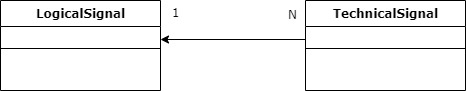
\includegraphics[scale=0.625]{images/class_diag_logical_technical_signal.jpg}
    \caption{LogicalSignal and TechnicalSignal class relationship}
    \label{fig:logical_technical_signal}
\end{figure}


Still regarding the signal mapping, an example can be put this way: A requirement signal within a clause evaluating the train speed (req. signal: <Train Speed>), would map to one technical signal (trainSpeed) of the system as the train speed is an atomic and singleton value throughout the train (i.e., it is not possible to have multiple train speeds). However, when checking whether the doors are closed and locked (req. signal <Doors enabled> is equal to false), checkings need to be performed for each door as there is on the train. In other words, if a train contains twenty doors, this requirement signal would actually map to as many signals as needed to represent all the door status. The signal mapping of these two requirement signals is presented on Table \ref{tab:signal_mapping}.

\begin{table}[h]
\caption{Signal mapping of train speed and door status}
    \footnotesize
    \centering
    
    \begin{tabular}{c c}
        \hline
        % --- ROW Header --- %
        \textbf{\textit{Logical Signal}} & 
        \textbf{\textit{Technical Signal}}
        \\ \hline  \\
        % --- ROW 1 --- %
        \begin{tabular}[c]{@{}c@{}} \textbf{\textit{ <Train speed> }} \end{tabular} & 
        BUS.ETH\_1.trainStatus.TrainSpeed \\
        \hline \\
        % --- ROW 2 --- %
        \begin{tabular}[c]{@{}c@{}} \textbf{\textit{ <Doors Enabled> }} \end{tabular} & 
            \begin{tabular}{@{}c@{}}
                BUS.ETH\_1.DCUStatus.C1ISDOEnCD\\ 
                BUS.ETH\_1.DCUStatus.C1ISDOEnAF\\ 
                BUS.ETH\_1.DCUStatus.C2ISDOEnCD\\ 
                BUS.ETH\_1.DCUStatus.C2ISDOEnAF\\ 
                BUS.ETH\_1.DCUStatus.C3ISDOEnCD\\ 
                BUS.ETH\_1.DCUStatus.C3ISDOEnAF\\ 
                BUS.ETH\_1.DCUStatus.C4ISDOEnCD\\ 
                BUS.ETH\_1.DCUStatus.C4ISDOEnAF\\ 
                BUS.ETH\_1.DCUStatus.C5ISDOEnCD\\ 
                BUS.ETH\_1.DCUStatus.C5ISDOEnAF\\ 
            \end{tabular}  \\
        \hline \\
        
    \end{tabular}
    \label{tab:signal_mapping}
\end{table}

The following requirement verbatim expresses the use of the signals previously mentioned. As per Table \ref{tab:signal_mapping}, each technical signal mapping to Doors enable provides the status of two doors aligned throughout the train, i.e., the status of the left and right door on the same train lenght point. It is also important to mention that when omitting any type o quantifier, the default behavior is the same as "for all" quantifier, hence, the verification of each door that maps to the requirement signal, the quantifier can act as a filter of the signals that go into the verification, this will be presented in detail on next section \ref{sec:method}.\\


\begin{Verbatim}[xleftmargin=12mm, numbers=left]
REQUIREMENT(REQ445-1, 2F03_Door_Functions, CCUS) 
{
	GIVEN <Doors enabled> is equal to false
		and <Train speed> is equal to 0;
	WHEN;
	THEN <Traction Safe> is set to true;
}
\end{Verbatim}

The corresponding signals are obtained by sending a request to the Signal Manager API, which is a centralised knowledge base that supports the information present on a requirement with additional data. This will be discussed in detail on next Section \ref{sec:method}.


\subsection{Test Generation}
%----------------------- Test Generation ----------------------------
\label{subsec:test_generation}

Test generator has two main roles: Translate each requirement signal into one or more software signals, and generate the combinatory explosion from the input signal values into test cases. Both procedures will be detailed on the next sub-sections.


\subsubsection{Test case generation and requirement coverage}
%----------------------- Test case generation ----------------------------
\label{subsubsec:test_cases}


For each requirement given as an input to this tool, \textit{Sesnando} extracts all the \textit{GIVEN} and \textit{WHEN} clauses. The evaluation of these combined predicates dictate the outcome of the requirement, in other words, dictate how the set of \textit{THEN} actions or effects on the train system should be observed (Figure \ref{fig:ti_er}). Those are defined as expected results. When both predicates evaluate to True, the \textit{THEN} actions defined by the requirement should be observed on the system, otherwise, they should be observed in its negative form or unrealised.\\

\begin{figure}[H]
    \centering
    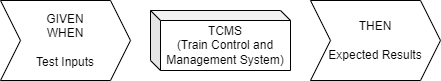
\includegraphics[scale=0.75]{images/In_out_TI_ER.png}
    \caption{Test Inputs and Expected Results}
    \label{fig:ti_er}
\end{figure}

Generated tests shall follow the the MCDC (Modified Condition/Decision Coverage) coverage criteria. MCDC is used in critical software development to ensure adequate testing. Essentialy, it states that every condition in a decision should independently affect the outcome of a decision and every decision and condition should take every possible outcome. MCDC is very similar to Active clause coverage regarding Logic Coverage \cite{intro_sw_testing}.
Meaning that, in the context of these works every predicate clause shall independently affect the outcome of this same predicate and for each clause and predicate every possible outcome is exercised.\\

It is important to mention that this requirement compiler supports predicate clauses separated by \textbf{AND} boolean operators. The reason being that the manufacturer prohibits the use of \textbf{OR} operators on system requirements by stating the following: \textit{"Multiple pre-conditions shall be linked only by AND, i.e. OR pre-conditions are forbidden."} on document \cite{tcms_req_guidelines}.\\

The use of \textit{Sesnando} on a different manufacturer project where Requirements with multiple boolean logic operator are used, require further developments on \textit{Sesnando} tool. This approach might include the reduction and simplification of the input logical expression and the application of a newly developed algorithm. These techniques have already been explored by this Github user (armin-montigny) \cite{armin-montigny_evaluation_2022}. However, \textbf{OR} operators are implicitly present on \textit{for at least} quantifiers as it will be shown further.\\

Considering the presented constrains, the outcome of a predicate is given by the Equation \ref{eq:eq1}.

\begin{equation}
    \text{Predicate Outcome} = \text{Clause1} \circ \text{Clause2} \circ \text{ClauseN}
    \label{eq:eq1}
\end{equation}


The observation of \textit{THEN} actions or effects are accorded to \textit{GIVEN} and \textit{WHEN} predicates combined, as such, this results in a similar Equation \ref{eq:eq2}

\begin{equation}
    \text{Realised THEN effects} = \text{GIVEN Predicate} \circ \text{WHEN Predicate}
    \label{eq:eq2}
\end{equation}


Meaning that a simple requirement REQ4661 containing one \textit{GIVEN} \textbf{AND} operator and a single \textit{WHEN} clause would result in a set of tests presented on Table \ref{tab:spec_single_and}.

\begin{Verbatim}[xleftmargin=12mm, numbers=left]
REQUIREMENT(REQ446-1, function, tcmsdevice) 
{
	GIVEN <SignalIn1> is equal to true
		and <SignalIn2> is equal to true;
	WHEN <SignalIn3> is equal to true;
	THEN <SignalOut1> is set to true;
}                                 
\end{Verbatim}

\begin{table}[h]
\caption{Test Spec for single AND}
    \footnotesize
    \centering
    
    \begin{tabular}{c c c c c}
        \hline
        % --- ROW Header --- %
        \textbf{\textit{Test step}} & 
        \textbf{\textit{SignalIn1}} & 
        \textbf{\textit{SignalIn2}} & 
        \textbf{\textit{SignalIn3}} & 
        \textbf{\textit{SignalOut1}}\\ \hline  \\
        
        % --- ROW 1 --- %
        \begin{tabular}[c]{@{}c@{}} \textbf{\textit{ 1 }} \end{tabular} & 
        0 & 
        1 &
        1 &
        0 \\
        \hline \\
        
        % --- ROW 2 --- %
        \begin{tabular}[c]{@{}c@{}} \textbf{\textit{ 2 }} \end{tabular} & 
        1 &
        0 &
        1 &
        0 \\
        \hline \\
       
        % --- ROW 3 --- %
        \begin{tabular}[c]{@{}c@{}} \textbf{\textit{ 3 }} \end{tabular} & 
        1 &
        1 &
        0 &
        0 \\
        \hline \\
        
        % --- ROW 4 --- %
        \begin{tabular}[c]{@{}c@{}} \textbf{\textit{ 4 }} \end{tabular} & 
        1 &
        1 &
        1 &
        1 \\
        \hline \\
        
    \end{tabular}
    \label{tab:spec_single_and}
\end{table}


Both predicates should evaluate to true in order to verify the expected results given by \textit{THEN} predicate. In other words, SignalInX will be written to the system, whereas SignalOutX will be read from the system and compared against expected results provided on Table \ref{tab:spec_single_and}.\\

For cases where a predicate clause contains a quantifier where the AND operator is implicit (e.g. For all), in order to check whether this clause affects the predicate outcome (as per MCDC), to evaluate the negative outcome of a predicate. all the quantifier signals are set to True, and the test steps start by negating each signal one-by-one as per Equation \ref{eq:for_all}. For cases where OR operator is implicit (e.g. For at least) the reverse scenario is applied as per Equation \ref{eq:for_at_least}. This is illustrated on Table \ref{tab:dbd_test_spec}. Further details of Test Generator is presented on Section \ref{sec:method}.

\begin{equation} \label{eq:for_all}
    \text{TechnicalSignal}[i] = False \quad \forall i \in \{0, 1, 2, \dots , n-1\}
\end{equation}

\begin{equation} \label{eq:for_at_least}
    \text{TechnicalSignal}[i] = True \quad \forall i \in \{0, 1, 2, \dots , n-1\}
\end{equation}

As an example, the requirement REQ4662 verbatim contains two signals whereas the <Train speed> maps to only one technical signal and the <Dragging Brake detected> maps to four signals. The clause containing the <Train speed> evaluates to true if the speed is above 3, so value 4 is used for the cases where the clause evaluates to true, and the value 3 is used when the clause should evaluate to false.

\begin{Verbatim}[xleftmargin=12mm, numbers=left]
REQUIREMENT(REQ446-2, 2F02_Traction_Braking, CCUS)
{
	GIVEN <Train speed> is greater than 3
	    and <Dragging Brake Detected> is equal to true 
	    for at least one brake in the Unit;
	WHEN;
	// Juridical Recording Unit
	THEN <JRU Dragging Brake Detected> is set to true;
}
\end{Verbatim}


Whereas, after the signal translation process, \textit{Sesnando} should retrieve multiple signals as many as there are brakes in the train unit. For simplicity and readability purposes, it will be assumed that Signal Manager returned four signals related to brakes on the train to the test generator. As it will be seen, the test specification will expand to a bigger test matrix. On the Equation \ref{eq:big_matrix}, O1 represents the output signal <JRU Dragging Brake Detected>, \textbf{m} represents the test step and \textbf{n}, the number of signals related to Requirement signal (a,b).

\begin{equation} \label{eq:big_matrix}
\text{O1} = 
Train Speed \circ Drag. Brake Det. = 
( b_i \cdot a_{ij}) = 
\begin{pmatrix} 
b_{1} \cdot  a_{11} & \cdots & a_{1n} \\
\vdots & \ddots & \vdots \\ 
 b_{m} \cdot  a_{m1} & \cdots & a_{mn} 
\end{pmatrix}
\end{equation}


So that, REQ446-2 would result in the test Table \ref{tab:dbd_test_spec}. Where Bk(x) represents each brake and TS representing the train speed technical signals. The expected result (JRU Dragging Brake Detected) for each test case is represented by JRU DBkDet.

\begin{table}[h]
\caption{Test Spec Dragging Brake Detected}
    \footnotesize
    \centering
    
    \begin{tabular}{c c c c c c c}
        \hline
        % --- ROW Header --- %
        \textbf{\textit{Test step}} & 
        \textbf{\textit{TS}} & 
        \textbf{\textit{Bk1}} & 
        \textbf{\textit{Bk2}} & 
        \textbf{\textit{Bk3}} & 
        \textbf{\textit{Bk4}} & 
        \textbf{\textit{JRU DBkDet}}\\ \hline  \\
        
        % --- ROW 1 --- %
        \begin{tabular}[c]{@{}c@{}} \textbf{\textit{ 1 }} \end{tabular} & 
        4 & 
        0 &
        0 &
        0 &
        0 &
        0 \\
        \hline \\
        
        % --- ROW 2 --- %
        \begin{tabular}[c]{@{}c@{}} \textbf{\textit{ 2 }} \end{tabular} & 
        3 &
        1 &
        0 &
        0 &
        0 &
        0 \\
        \hline \\
       
        % --- ROW 3 --- %
        \begin{tabular}[c]{@{}c@{}} \textbf{\textit{ 3 }} \end{tabular} & 
        4 &
        1 &
        0 &
        0 &
        0 &
        1 \\
        \hline \\
        
        % --- ROW 4 --- %
        \begin{tabular}[c]{@{}c@{}} \textbf{\textit{ 4 }} \end{tabular} & 
        4 &
        0 &
        1 &
        0 &
        0 &
        1 \\
        \hline \\
        
        % --- ROW 5 --- %
        \begin{tabular}[c]{@{}c@{}} \textbf{\textit{ 5 }} \end{tabular} & 
        4 &
        0 &
        0 &
        1 &
        0 &
        1 \\
        \hline \\
        
        % --- ROW 6 --- %
        \begin{tabular}[c]{@{}c@{}} \textbf{\textit{ 6 }} \end{tabular} & 
        4 &
        0 &
        0 &
        0 &
        1 &
        1 \\
        \hline \\
        
    \end{tabular}
    \label{tab:dbd_test_spec}
\end{table}

Table \ref{tab:dbd_test_spec}, is is the result of the logical expression:\\
$((TS > 3) \land (Bk1 \lor Bk2 \lor Bk3 \lor Bk4))$\\
It can be observed that, as per MCDC Coverage criteria, each clause takes every possible outcome, every decision (predicate) takes every possible outcome and each condition (clause) affects every possible decision outcome. This process is fully automated within the Test Generator module of \textit{Sesnando}.


\subsubsection{Signal Translation and quantifier signal attributes}
%----------------------- Signal Translation ----------------------------
\label{subsubsec:sub_signal_translation}

\textit{Sesnando} extracts every requirement signal from the input requirement and asks the Signal manager for its corresponding Technical signals. This is achieved by calling a Signal Manager API endpoint \\
(e.g., \textcolor{black}{https://<IP\_Address>:5001/api/signal/<LogicalSignal>}).\\

When a \textit{Logical signal} is not found, \textit{Sesnando} will report an error message to the user for the current requirement, as the signal must be added to the Database.

When a requirement is applied to a multiple set of components of the same type on the system (Doors, Brakes, Axles), \textit{Sesnando} looks to test these components individually (See Section \ref{subsubsec:test_cases}), when a requirement instructs to do so, this is achieved through the use of quantifiers as previously presented on Section \ref{tab:signal_mapping}.

All the train elements and attributes can be presented on an hierarchical format. Figure \ref{fig:hier_elem_attr} presents this said hierarchy and some of their attributes.

\begin{figure}[h]
    \centering
    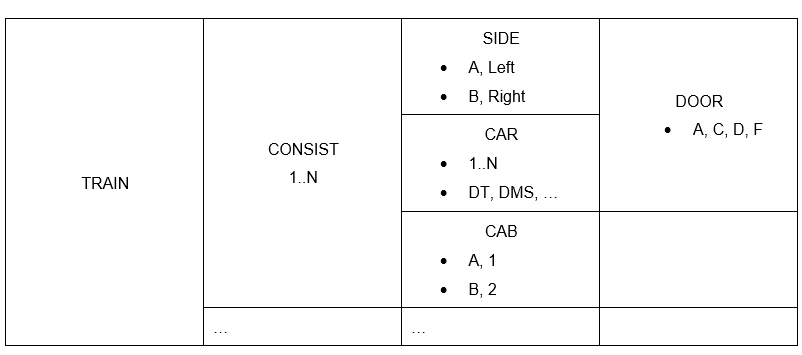
\includegraphics[width=\textwidth]{images/hier_elems_attrs.PNG}
    \caption{Table train elements and attributes (excerpt)}
    \label{fig:hier_elem_attr}
\end{figure}

Element attributes are important during the generation of the test cases. There is a train functionality that, regarding the location of train, the Driver might not be allowed to open the doors for a given side. This behavior is presented on the following requirement verbatim.


\begin{Verbatim}[xleftmargin=12mm, numbers=left]
REQUIREMENT(REQ446-3, function, tcmsdevice) 
{
	GIVEN <Door Open Permit> is equal to true for one side;
	WHEN <Driver Desk Door Open> is equal to true 
	    for the same side;
	THEN <TCMS command door open> is set to true 
	    for the same side;
}
\end{Verbatim}

The signals on Figure \ref{fig:hier_elem_attr} are an extract from a test script related to <Door open permit>. These are used as an example to present the signal attributes.

\begin{figure}[H]
    \centering
    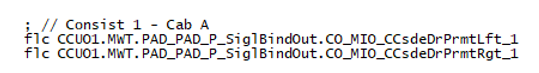
\includegraphics[width=\textwidth]{images/door_prmt.PNG}
    \caption{Door open permit signals}
    \label{fig:hier_elem_attr}
\end{figure}

The signal attributes from signals on Figure \ref{fig:hier_elem_attr} are presented on Figure \ref{fig:door_perm_sig_attr}, which are extracted from the project documentation (e.g. ICDs and ISLs) and are then populated on Signal manager to support the generation of tests by \textit{Sesnando}.

\begin{figure}[H]
    \centering
    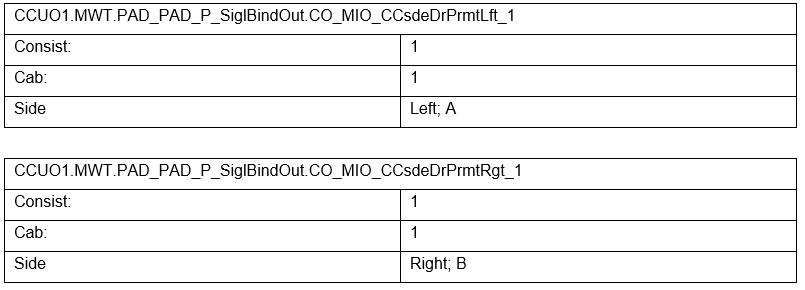
\includegraphics[width=\textwidth]{images/signal_attr_dp.PNG}
    \caption{Door open permit signals attributes}
    \label{fig:door_perm_sig_attr}
\end{figure}


So that, REQ4662 would result in the test Table \ref{tab:for_the_same_test_spec}. Where DOPlft and DOPRgt represents <Door Open Permit> technical signals, DDDOLft and DDDORgt <Driver Desk Door Open> the technical signal for the Driver Door open command. The expected result (<TCMS command door open>) for each test case is represented by TCMSDOLft and TCMSDORgt.

\begin{table}[H]
\caption{Test Spec - for the same quantifier}
    \footnotesize
    \centering
    
    \begin{tabular}{c c c c c c c}
        \hline
        % --- ROW Header --- %
        \textbf{\textit{Test step}} & 
        \textbf{\textit{DOPlft}} & 
        \textbf{\textit{DOPRgt}} & 
        \textbf{\textit{DDDOLft}} & 
        \textbf{\textit{DDDORgt}} & 
        \textbf{\textit{TCMSDOLft}} & 
        \textbf{\textit{TCMSDORgt}}\\ \hline  \\
        
        % --- ROW 1 --- %
        \begin{tabular}[c]{@{}c@{}} \textbf{\textit{ 1 }} \end{tabular} & 
        0 & 
        1 &
        0 &
        0 &
        0 &
        0 \\
        \hline \\
        
        % --- ROW 2 --- %
        \begin{tabular}[c]{@{}c@{}} \textbf{\textit{ 2 }} \end{tabular} & 
        1 &
        0 &
        0 &
        0 &
        0 &
        0 \\
        \hline \\
       
        % --- ROW 3 --- %
        \begin{tabular}[c]{@{}c@{}} \textbf{\textit{ 3 }} \end{tabular} & 
        1 &
        1 &
        0 &
        0 &
        1 &
        0 \\
        \hline \\
        
        % --- ROW 4 --- %
        \begin{tabular}[c]{@{}c@{}} \textbf{\textit{ 4 }} \end{tabular} & 
        0 &
        0 &
        0 &
        1 &
        0 &
        0 \\
        \hline \\
        
        % --- ROW 5 --- %
        \begin{tabular}[c]{@{}c@{}} \textbf{\textit{ 5 }} \end{tabular} & 
        0 &
        0 &
        1 &
        0 &
        0 &
        0 \\
        \hline \\
        
        % --- ROW 6 --- %
        \begin{tabular}[c]{@{}c@{}} \textbf{\textit{ 6 }} \end{tabular} & 
        0 &
        0 &
        1 &
        1 &
        0 &
        1 \\
        \hline \\
        
    \end{tabular}
    \label{tab:for_the_same_test_spec}
\end{table}


\textit{Sesnando} internally divides the testing for both sides into two test cases (1-3,4-6), for left and right. In other words, for as many sides there are on the train.
The quantifier \textit{for the same} is under a conceptual phase and hasn't been fully implemented yet.


\subsection{Signal Manager}
%----------------------- Signal Manager ----------------------------
\label{subsec:signal_manager}

Ideally, \textit{Signal Manager} should run on a remote server where the testing information is centralized. The main benefits of this approach is that every tester, developer or project stake-holder can contribute to develop a solid knowledge base to sustain the test generation from \textit{Sesnando Compiler} instance.\\

\textit{Signal Manager} can be accessed trough a Web Interface running on port 5001. From there, the user is able to edit Technical signals (Software signals) which can be mapped to the corresponding Logical Signals (Requirement Signals) as well as add relevant data like attributes and states. See (Fig. \ref{fig:signal_manager_pibs})

\begin{figure}[H]
    \centering
    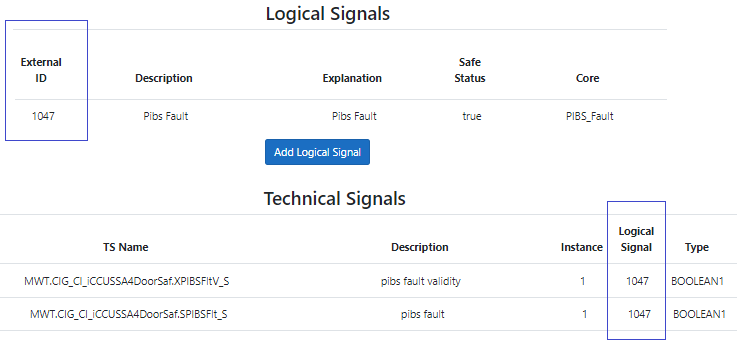
\includegraphics[width=\textwidth]{images/signal_manager_signals_pibs.PNG}
    \caption{Signal Manager PIBS Signal Mapping example}
    \label{fig:signal_manager_pibs}
\end{figure}

The Figure \ref{fig:signal_manager_pibs} is an excerpt from the \textit{Signal Manager} interface. It can be seen that a set of technical signals are mapped to a Logical Signal trough an Id value. A Technical signal might accept several attributes, e.g., a door \textit{Side} or Car location within the train or a state, e.g., Open, Released, Closed, that might be represented through an integer number, this is defined from the original requirement, e.g., "Given <Door status> is equal to Released".


\subsection{Test Designer}
%----------------------- Test Designer ----------------------------
\label{subsec:test_designer}

The main goal of \textit{Test Designer} is to display the generated test specification to the user. The user is able to modify it as intended and from there, generate a test script. This interface is presented on the next image (Fig. \ref{fig:test_designer_interface}).

\begin{figure}[H]
    \centering
    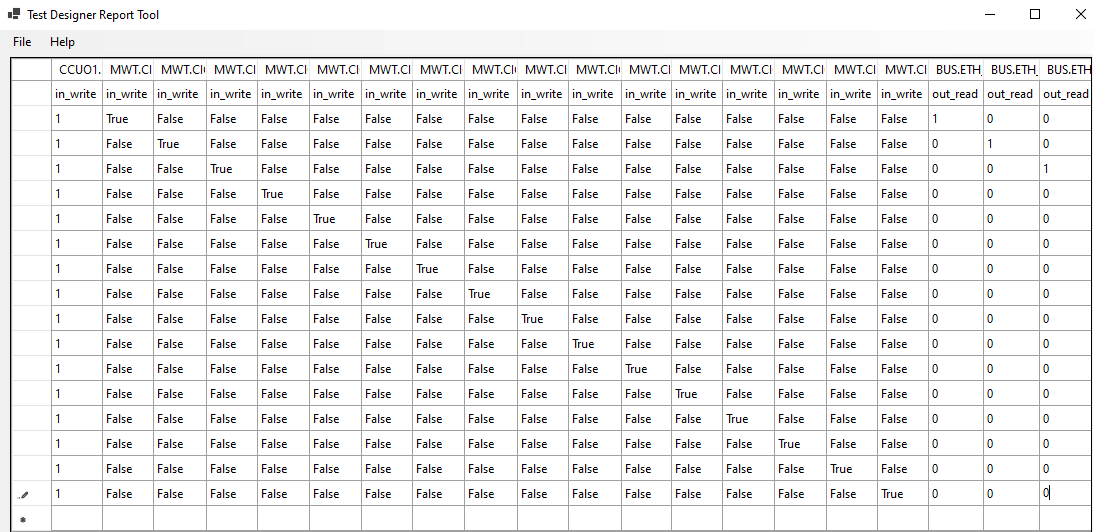
\includegraphics[width=\textwidth]{images/test_designer.PNG}
    \caption{Test Designer Interface}
    \label{fig:test_designer_interface}
\end{figure}

The above image (Fig. \ref{fig:test_designer_interface}) is the result of a scalar requirement signal evaluating to int value "1" combined with an \textit{AND} operator to a quantifier requirement signal. Tests are executed from top to bottom.
The first row of the table corresponds to the software technical signal, the second row defines the direction of the signal as:

\begin{itemize}
    \item in\_write - The value to be \textit{forced} on the corresponding technical signal.
    \item out\_write - The expected results according the test inputs from the left input columns.
\end{itemize}

Test designer test tables are representations of test specifications presented on Section \ref{subsec:test_generation}.


\subsubsection{Generated Artifacts and test execution}
%----------------------- Generated Artifacts ----------------------------
\label{subsubsec:generated_artifacts}

After visualising and reviewing the test specification on the test designer, the tester will be able to export it into a test script compatible with the test execution tool. This feature can be located by navigating to "File -> Export to test script". At this moment \textit{Sesnando} only supports one script type but it is intended that the user interface could be extended to support multiple script types as needed.\\
With this, it is intended to demonstrate a complete end-to-end lifecycle, from requirements to test execution. Next, is a tool that allows the observation of the internal states of a simulated train in operation (Fig. \ref{fig:test_environment})

\begin{figure}[H]
    \centering
    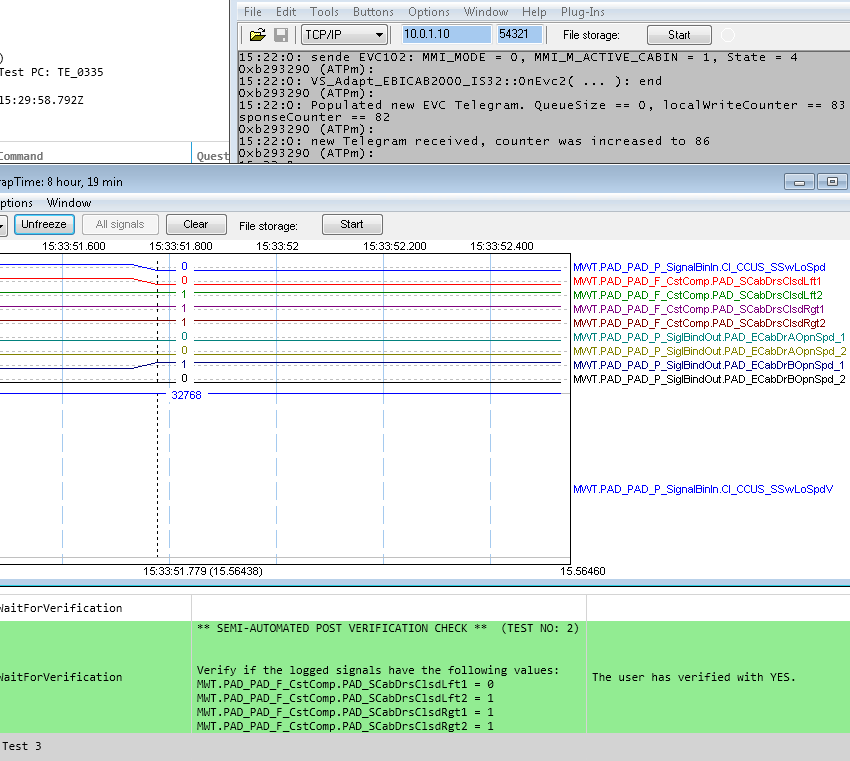
\includegraphics[width=\textwidth]{images/test_environment.png}
    \caption{Test Environment}
    \label{fig:test_environment}
\end{figure}

The validation facility (which might be in a form of Test Rack or a local testers' computer, Section \ref{sec:current_procedures}) loads the script generated from \textit{Sesnando}. On a simple operation, the signal values start to be set on the software to produce the desire outcomes. The real-time value of every software signal through the test time-span can be observed on the multi-chart present on the software tool (Fig. \ref{fig:test_environment}). This also demonstrates that \textit{Sesnando} is able to generate test scripts from the input requirements that are compatible with the presented test environment.





    \section{Method}
%----------------------- Method ----------------------------
\label{sec:method}

This section describes the steps and decisions taken towards the development of Sesnando. The concepts presented here are the result of the study of the state of the art and internal discussions with Project Advisors.


\subsection{Resource Analysis}
%----------------------- Resource Analysis ----------------------------
\label{subsec:resource_analysis}

This section presents the analysis procedures towards the available resources, namely, requirements sets. The Railway project used for this study stores its requirements on a Requirement Management Tool. Those requirements have been exported and analysed to extract relevant knowledge from them towards building a solid grammar that could satisfy these requirements logic.\\

It was not feasible to analyse such requirements one-by-one due to their number, so a tool has been developed to extract the needed data. First, the requirements have been exported in chunks of Excel files, but later, this same tool was able to directly access the requirement repository.

The requirement analysis tool has been developed using the following libraries.

\begin{itemize}
    \item pandas - For importing requirement files, data storage and data analysis.
    \item nltk - Natural Language Toolkit for data analysis.
    \item matplot - Data visualisation.
    \item xlswriter - To persist processed data.
\end{itemize}

The principal analysis taken was in the fields on the contiguous sequence and main requirement structures, for this, several models on N-Grams and Skip-grams have been generated.\\
N-gram model analysis are widely used in computational linguistics and communication theory such as Natural Language Processing (NLP) \cite{broder_syntactic_1997}.\\

The techniques to export the best N-gram models relied on arbitrary values and \textit{trial and error}. N-gram models above the value of 10 started to produce several repeating sequences, so the model analysis sat between the values of 2 and 10. Next is one of the N-gram Model where N = 10.

% width=\textwidth
\begin{figure}[H]
    \centering
    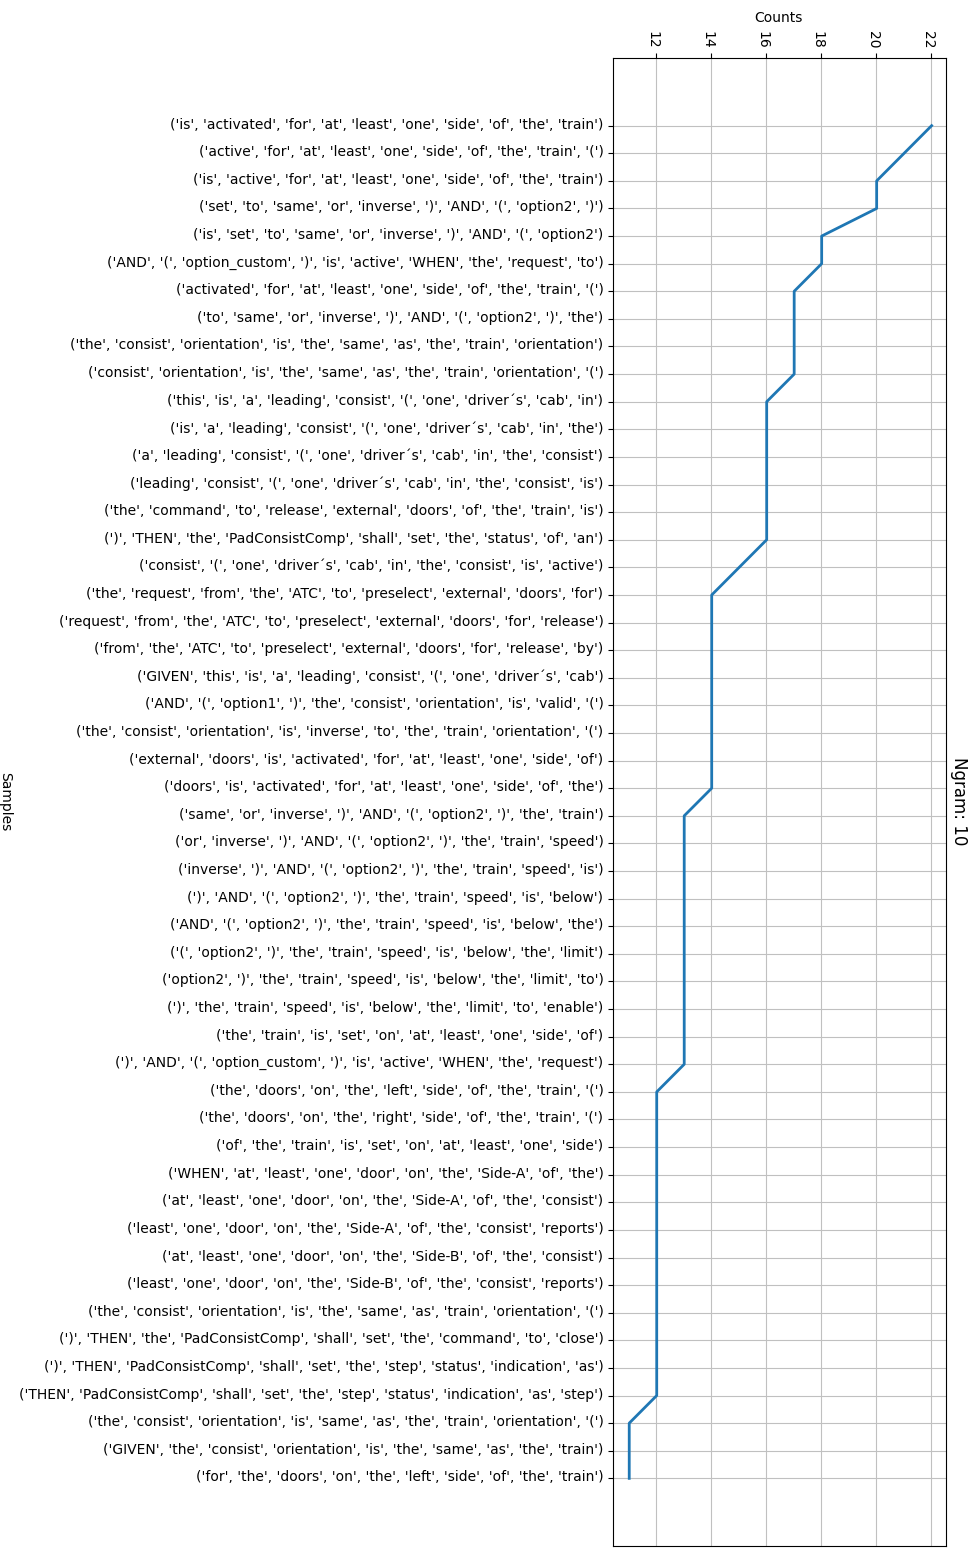
\includegraphics[scale=0.6]{images/n_gram10_cut.png}
    \caption{N-gram Model, N = 10}
    \label{fig:n_gram_model_10}
\end{figure}

The results of this analysis expressed the need of using boolean operators such as "AND" and "OR". Signal states such as "is active". Quantifiers containing their component/attribute and scope, as in "for at least one side of the train" and the \textit{THEN} condition in the form of "THEN the \textit{AUTOR} shall set the Requirement signal to \textit{VALUE}".
These have been used to define the requirements grammar, as it will be seen on next section (\ref{sec:def_req_grammar}).


\subsection{Defining the requirements grammar}
%----------------------- Defining the requirements grammar ----------------------------
\label{sec:def_req_grammar}

As the grammar lexer set has been identified it was then necessary to define an Abstract Syntax tree. It is known that \textit{GIVEN}, \textit{WHEN} and \textit{THEN} are the main predicates that define the skeleton of a requirement, thus, each predicate should implement its own Condition tree.\\
There are widely known libraries to support the building of a grammar, such as Flex and Bison \cite{levine_flex_2009}, however, flex and bison only work with C++ programs and Antlr works with a number of different languages \cite{antlr_site}, hence the choice of \textit{Antlr} library to support the development of this grammar. \textit{GIVEN}, \textit{WHEN} and \textit{THEN} are represented in the form of a Logical Expression that can be derived into child classes, given the lexer type. The representation of the syntax tree is presented on Fig. \ref{fig:ast_class_diagram}.

% 
\begin{figure}[H]
    \centering
    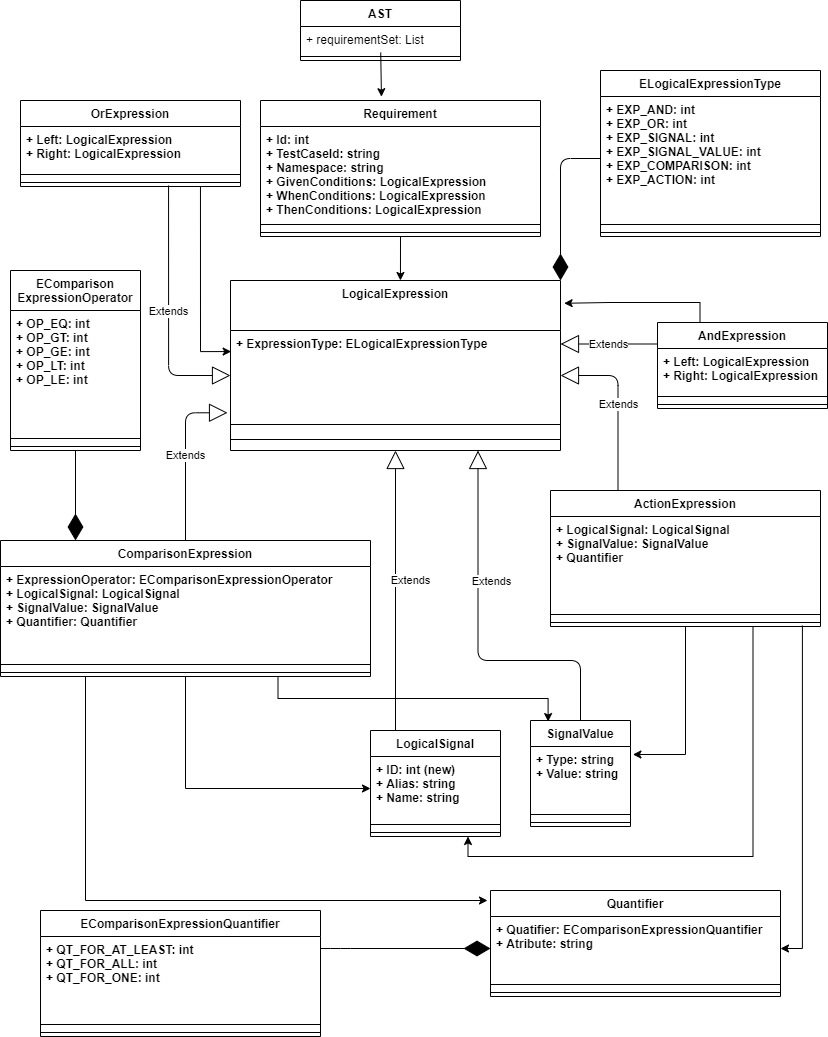
\includegraphics[width=\textwidth]{images/grammar_class_diagram.drawio.png}
    \caption{AST Class Diagram}
    \label{fig:ast_class_diagram}
\end{figure}

The defined grammar also supports the use of comments in the input file in the format of line comment or block-comment, "//" and "/**/" respectively.\\
The AST on Figure \ref{fig:ast_class_diagram} implements a list of requirements with as many as uncommented on the input file. The type of each expression is given by the ELogicalExpressionType enumerator. \textit{AndExpression} and \textit{OrExpression} are the defined boolean operators, however, Sesnando will report a warning message when an "OR" is used, as it usage is not advised according to Railway original requirement guidelines. A \textit{ComparisonExpression} is used for \textit{GIVEN} and \textit{WHEN} predicates and the \textit{ActionExpression} on \textit{THEN} predicates, as they define the output actions of a requirement, i.e., the expected results.


\subsection{Test case generation}
%----------------------- Command Line Inputs ----------------------------
\label{subsec:def_test_case_gen}

Functional or behavioral testing generates an output based on the given inputs and determines if the system is functioning correctly as per the specifications \cite{jorgensen_software_2011}.\\

\begin{figure}[H]
    \centering
    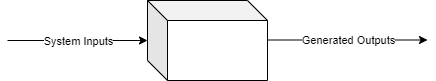
\includegraphics[scale=0.65]{images/functional_inputs_outputs.png}
    \caption{Blackbox testing}
    \label{fig:blackbox_testing}
\end{figure}

The Cause-Effect Graph (CEG) technique is a black-box method that considers only the desired external behavior of a system. It is also the only black-box test design technique that considers combinations of causes of system behaviors \cite{nursimulu_cause-effect_1995}.

It can be assumed that each requirement in the form of \textit{GIVEN WHEN THEN} dictate a cause effect, as such, a collection of requirements cover a certain area of the software.\\

Robustness testing is the ability of a software to keep an "acceptable" behaviour expressed in terms of \textit{robustness requirements}, in spite of exceptional or unforeseen execution conditions, such as communication failures, degraded modes, etc. \cite{khendek_model-based_2005}. Robustness requirements are within the set of pilot Railway project requirement collection, thus, it can be stated that by testing each requirement within the scope of this Railway project, Requirement coverage is achieved.\\

As previously stated, a Requirement \textit{GIVEN} predicate defines the requirement or test pre-conditions, and \textit{WHEN} defines the requirement trigger conditions and implies an internal state change, thus, by invalidating such requirement conditions does not guarantee that the system or software internal state is changed and system behaves otherwise.\\

For a requirement that implies a change of a state, it needs to verify whether different causes or conditions do not conflict with the current state change. An hypothetically example can be observed on the following image (Fig. \ref{fig:door_isolation}).\\

\begin{figure}[H]
    \centering
    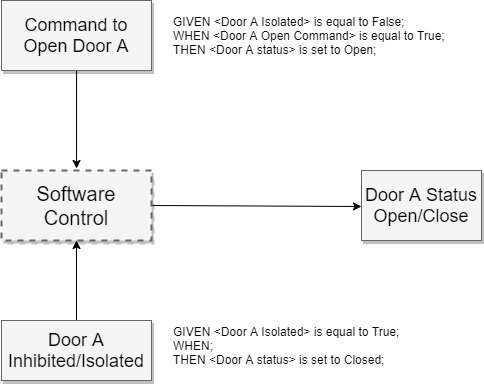
\includegraphics[scale=0.6]{images/isolation_diagram.png}
    \caption{Internal State change - Door Isolation}
    \label{fig:door_isolation}
\end{figure}

In the above example (Fig. \ref{fig:door_isolation}), the Door Isolation requirement when evaluating to true needs to guarantee that the Door close state is assured, however, it cannot be stated otherwise, i.e., that door state would be set to Open when Isolation is not present, as this is given by the Door Open command, this requirement needs to verify that there are no other conditions conflicting or affecting the desired results, hence, the verification of the presence of the isolation.

In summary, \textit{Sesnando} generates test cases according to requirement instructions.\\

On an additional note, an internal survey has revealed that conflicting requirements are very unlikely to happen, however, for cases where it does, those should be found on \textit{upper} vehicle/system level testing.\\

\textcolor{red}{Provision - Se o Sesnando suportar opcionalmente negative tests a partir de AND requirements, ou seja, quando não existem requisitos de robustez, falar disso aqui.}\\


\subsection{Signal Manager Architecture}
%----------------------- Signal manager ----------------------------
\label{subsec:method_signal_manager}

As previously stated, it is intended that Signal Manager could be run as a detached service from the local compiler solution. This would allow that every tester, developer or involved user could contribute to the growth of information in it, such that every piece of testing information would be added only once, thus, the Test Generator accesses this remote repository in order to generate its tests, contributing to efficiently reduce the efforts needed, otherwise, every signal would need to be added as much as every existing localhost solutions.\\
The Signal manager acts as a Web Service and serves the Signal Manager through a REST API. There are several endpoints to consult, edit and create additional signals on the database. The purpose of these API Endpoints is not only to support Test Generator, but also the management of the signal data without the need of accessing the web user interface, e.g, automating the import of huge chunks of signal data. The Signal Manager contains fourteen database tables which supports the logic described throughout this report. An excerpt of this database can be observed on Fig. ~\ref{fig:db_signal_manager}.

\begin{figure}[H]
    \centering
    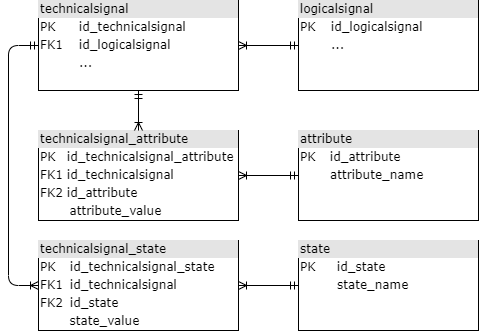
\includegraphics[scale=0.7]{images/signal_manager.png}
    \caption{Signal Manager DB Architecture (Excerpt)}
    \label{fig:db_signal_manager}
\end{figure}

A Logical Signal maps to one or more technical signals and a technical signal supports multiple attributes and states. A train Brake can be used as an example, as a possible attribute would be the location of this Brake within the train (Car=1,2..N) and its Axle (Axle=1..2), given that a train Car might contain two axles and a possible state would be whether this brakes are released or not (state="released", "not released") the latter usually maps to an integer value to represent the state, i.e, 1 or 0. This information is cross-checked on the Test Generator to process the correct technical signals according to the requirement information.


\subsection{Test Designer}
%----------------------- Signal manager ----------------------------
\label{subsec:method_test_designer}

The main benefits the test designer is the ability of the user to visualise the contents the test specification. By default, the test generator persists the test specification on a CSV file, so, without a Graphical User Interface, the user would have to rely on external tools in order to review it. In other words, the Test Designer loads the CSV contents into a grid-view where several operations might be executed, such as editing and saving this CSV file or generate test scripts.

\chapter{Results}
\label{ch:5}

Results

\addcontentsline{toc}{chapter}{Conclusions and Future Work}
\chapter*{Conclusion}

Conclusions


% Bibliografia automática
\bibliographystyle{unsrt}
\bibliography{bibliografia}

\appendix
\chapter*{Appendix}

\section{Benchmarking}
\label{apx:section_apx}

The requirement REQ442-2 from Section \ref{subsec:sesnando_input} has been benchmarked using the Eclipse IDE with ANTLR4 IDE 0.3.6 from the marketplace, resulting in the Figure \ref{fig:req_parse_tree}. Benchmark results are as follows:

\begin{table}[H]
\caption{ANTLR Grammar Profiler}
    \footnotesize
    \centering
    \begin{tabular}{c c c}
        \hline
        \textbf{\textit{Measurement}} & \textbf{\textit{Value}}\\ \hline
            &  \\
     \begin{tabular}[c]{@{}c@{}} \textbf{\textit{Input}} \textbf{\textit{Size}}\end{tabular}  & 198 chars, 6 lines  \\ \hline
        &   \\ 
       \textbf{\textit{ Number of Tokens}} & 34  \\ \hline
        &   \\
        \textbf{\textit{Parse Time (ms)}} & 2268 \\ \hline
            &   \\
        \textbf{\textit{Prediction Time (ms)}} & 0,711 = 31.36\%  \\ \hline
            &   \\
       \textbf{\textit{Lookahead Burden}} & 53/34 = 1.56  \\ \hline
        &  \\
       \textbf{\textit{DFA Cache miss rate}} &  \begin{tabular}[c]{@{}c@{}} 43/53 = 81.13\% \end{tabular}  \\ \hline
    \end{tabular}
    \label{tab:grammar_benchmark}
\end{table}

\end{document}